\section{Implementazioni OpenMP}
Per parallelizzare l'algoritmo usando \emph{OpenMP} sono state realizzate alcune versioni in modo da valutare l'efficacia di diversi approcci o strumenti.
In particolare è risultato evidente che impostando la variabile d'ambiente \texttt{OMP\_PROC\_BIND=true} si ottengono risultati migliori sia dal punto di vista dell'efficienza, ma soprattutto da quello della \textbf{ripetibilità}: senza l'utilizzo della variabile esecuzioni successive dello stesso programma terminavano spesso in tempi molto diversi.

Analizzando il funzionamento dell'algoritmo si può dire che ad ogni iterazione viene aggiunto all'\emph{hull} il punto più esterno rispetto all'ultimo inserito $P_l$;
$P_a$ è più esterno di $P_b$ se la spezzata $P_lP_aP_b$ è orientata in senso orario.

È possibile utilizzare il \textbf{pattern reduction} ad ogni iterazione per scegliere il punto più esterno, utilizzando la direttiva \texttt{reduce} di OMP.  
Per poter eseguire la \emph{reduction} su punti e per gestire il contesto necessario ai confronti (ovvero il punto precedente nel convex hull),
è stata dichiarato un operatore personalizzato con la direttiva \texttt{\#pragma omp declare reduction}.

Di seguito è riportato lo speedup ottenuto parallelizzando la ricerca del prossimo punto $P_next$ usando la direttiva \texttt{reduce} con l'operatore sopra citato:

\begin{figure}[h]
    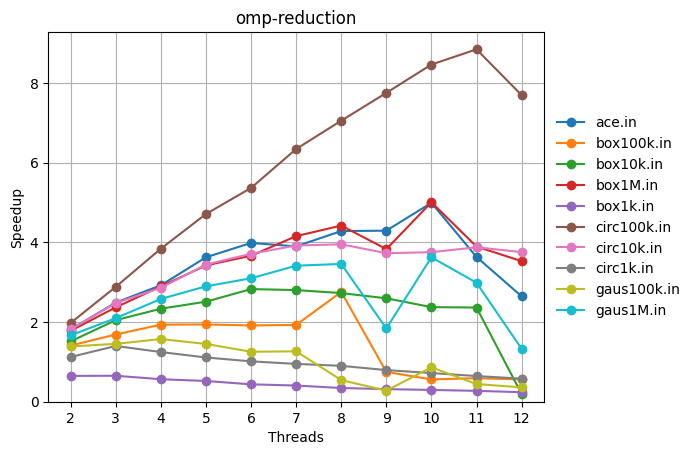
\includegraphics[width=\textwidth]{omp-reduction}
    \centering
\end{figure}
